\documentclass{article}

\usepackage{ocencfd}
\usepackage{geometry}
\usepackage{graphicx}
\usepackage{float}
\usepackage{amsfonts}
\usepackage{mathrsfs}
\usepackage{mwe}
\usepackage{subfig}

\title{Introduction to Deep Learning\\Assignment 2} % Sets article title
\author{\textbf{Group 53}\\Chenyu Shi (s3500063); Shupei Li (s3430863); Shuang Fan (s3505847)} % Sets authors name
\documentID{Introduction to Deep Learning Assignment 2} %Should be alphanumeric identifier
\fileInclude{} %Names of file to attach
\date{\today} % Sets date for publication as date compiled

\geometry{a4paper, left=2cm, right=2cm, top=2cm, bottom=2cm}

% The preamble ends with the command \begin{document}
\begin{document} % All begin commands must be paired with an end command somewhere

\maketitle % creates title using information in preamble (title, author, date)

\section*{Task 1}

\section*{Task 2}

\section*{Task 3}
\setcounter{section}{3}
\subsection{Datasets}
We use two datasets in Task 3. Firstly, we explore the performance of different model architectures and the effects of different parameters with MNIST data. After that, we leverage the power of generative models on Butterfly \& Moth data. \par
We directly call Tensorflow API to download the MNIST dataset. However, the original dataset is also available on \url{https://deepai.org/dataset/mnist}. MNIST dataset contains 70,000 grayscale images (28 $\times$ 28 $\times$ 1), whose content is handwritten numbers. \par
Butterfly \& Moth is an open source dataset on Kaggle. There are 13,639 RGB images (224 $\times$ 224 $\times$ 3) composed of 100 butterfly or moth species. Link of the dataset is \url{https://www.kaggle.com/datasets/gpiosenka/butterfly-images40-species?resource=download}.

\subsection{Experimental Set-up}
All experiments are deployed on two servers. Server 1 has an Intel(R) Xeon(R) Platinum 8358P CPU and a RTX A5000 GPU, while server 2 has an Intel(R) Xeon(R) E5-2680 v4 CPU and a TITAN Xp GPU. Table \ref{tab:3-hyper} summarizes the hyperparameter values in the experiments. The following describes the process of our experiments.
\begin{table}[!ht]
    \centering
    \caption{Hyperparameter Settings}
    \label{tab:3-hyper}
    \begin{tabular}{lll}
        \toprule
        \textbf{Parameter} & \textbf{Value} & \textbf{Meaning}\\
        \midrule
        cae\_latent\_dim & 32 & Dimensions of the latent space in CAEs.\\
        cae\_epoch & 10 & The number of training epochs in CAEs.\\
        vae\_latent\_dim & 32 & Dimensions of the latent space in VAEs.\\
        vae\_epoch & 20 (MNIST) / 100 (Butterfly \& Moth) & The number of training epochs in VAEs.\\
        gan\_latent\_dim & 256 & Dimensions of the latent space in GANs.\\
        gan\_epoch & 20 (MNIST) / 250 (Butterfly \& Moth) & The number of training epochs in GANs.\\
        \bottomrule
    \end{tabular}
\end{table}

\subsubsection{MNIST}
We modify the model architecture to decrease the model complexity and match the data better. Specially, we build the basic convolutional network with four Conv2D layers and construct the basic deconvolutional network with one Conv2DTranspose layer. Figure \ref{fig:3-model} illustrates our model settings. There is no need to resize the images due to the modification of the model.
\begin{figure}[!ht]
    \centering
    \subfloat[Convolutional network]{%
        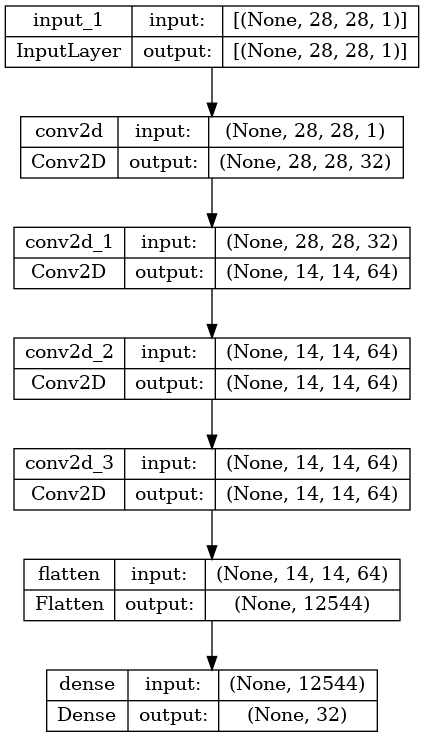
\includegraphics[height=6cm, width=6cm]{./fig/conv.png}%
        \label{fig:conv}%
        }%
        \hspace{0.8cm}
    \subfloat[Deconvolutional network]{%
        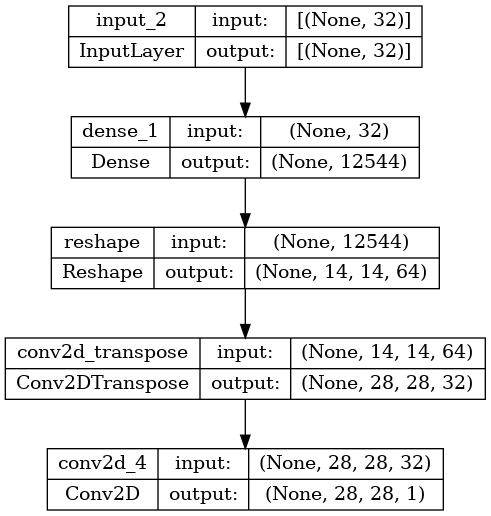
\includegraphics[height=6cm, width=7cm]{./fig/deconv.png}%
        \label{fig:deconv}%
        }%
    \caption{Model Structure}
    \label{fig:3-model}
\end{figure}

\subsubsection{Butterfly \& Moth}
We rescale the images to 64 $\times$ 64 $\times$ 3 and directly apply the model architecture provided in the notebook when working with Butterfly \& Moth data.

\subsection{Results}
\textbf{CAEs}. Figure \ref{fig:3-cae} shows the reconstructed images from CAEs. It is easy to see that CAEs have captured the main features in the original images.
\begin{figure}[!ht]
    \centering
    \subfloat[MNIST: Original Images]{
        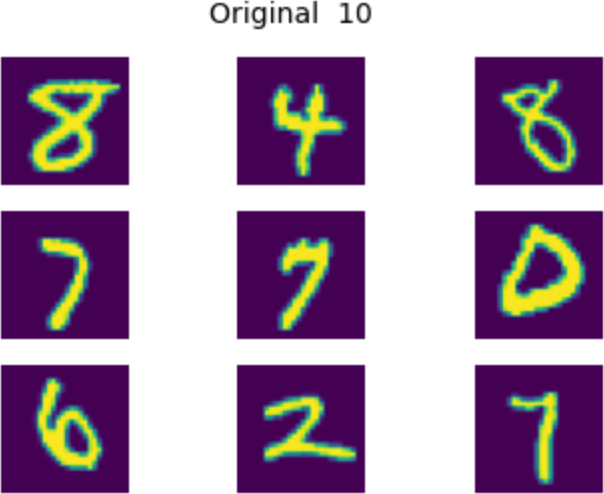
\includegraphics[width=5.6cm]{./fig/mnist-cae-ori.png}
    }
    \hspace{1cm}
    \subfloat[MNIST: Reconstructed Images]{
        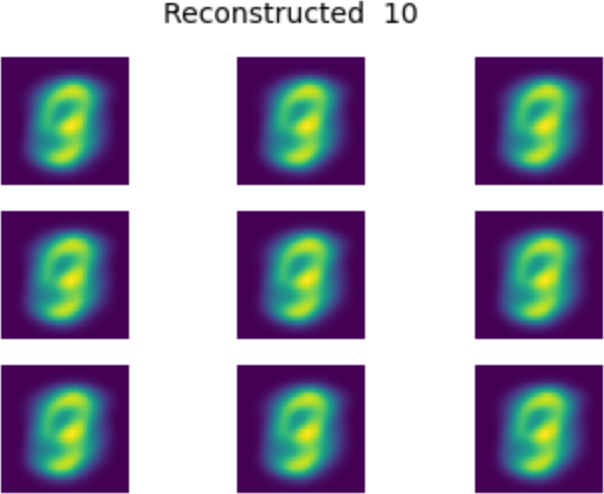
\includegraphics[width=5.6cm]{./fig/mnist-cae-re.png}
    }
    \\
    \subfloat[Butterfly \& Moth: Original Images]{
        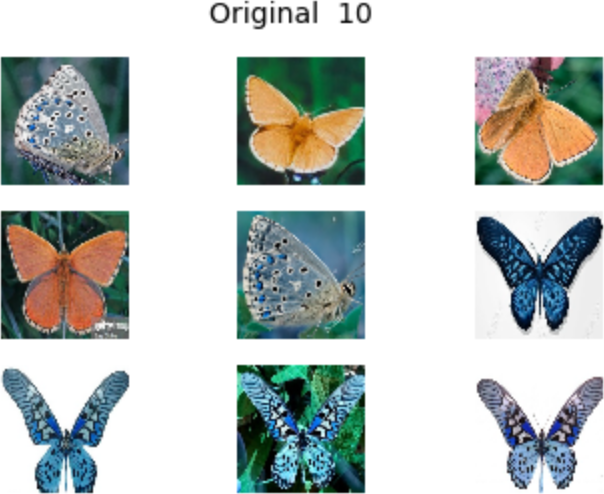
\includegraphics[width=5.6cm]{./fig/bm-cae-ori.png}
    }
    \hspace{1cm}
    \subfloat[Butterfly \& Moth: Reconstructed Images]{
        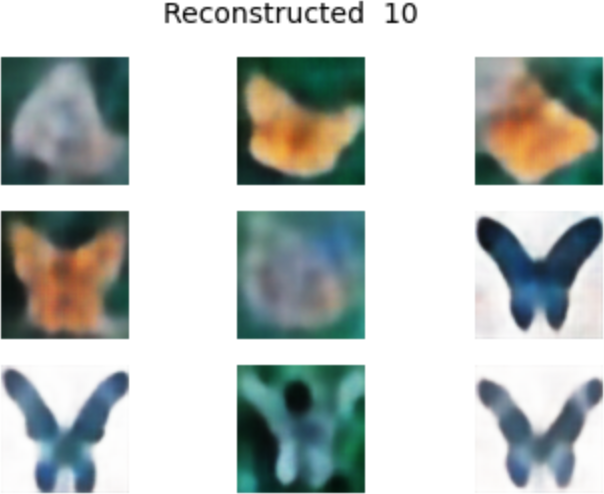
\includegraphics[width=5.6cm]{./fig/bm-cae-re.png}
    }
    \caption{Results of CAEs}
    \label{fig:3-cae}
\end{figure}
\par~\\
\textbf{VAEs}. We explore the learned latent space with linear interpolation technique. Firstly, we sample a point from the latenty space by generating its coordinates from a standard normal distribution. Then, we change one or two coordinates along the straight line in the latent space, while keep other coordinates unchanged. For MNIST dataset, we apply linear interpolation on the 10th and 27th coordinates simultaneously, which are related to the shape of the number. Figure \ref{fig:vae-mnist} shows the visualization results.
\begin{figure}[!ht]
    \centering
    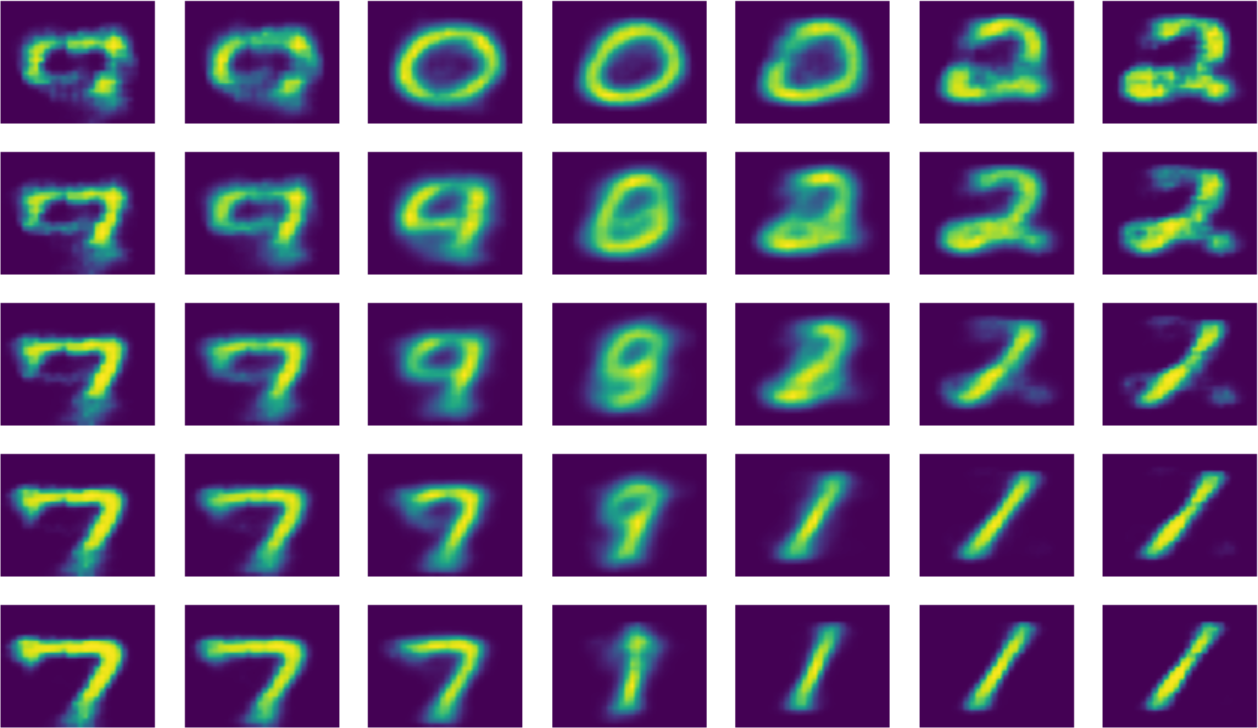
\includegraphics[width=10cm, height=5cm]{./fig/mnist-vae.png}
    \caption{VAEs: MNIST Data}
    \label{fig:vae-mnist}
\end{figure}
As for Butterfly \& Moth data, we linearly interpolate the 6th and 29th coordinates, whose outputs are presented in Figure \ref{fig:vae-bm}. According to Figure \ref{fig:vae-bm}, the 6th coordinate is related to the color of wings, while the 29th coordinate is concerned with the width of wings.
\begin{figure}[!ht]
    \centering
    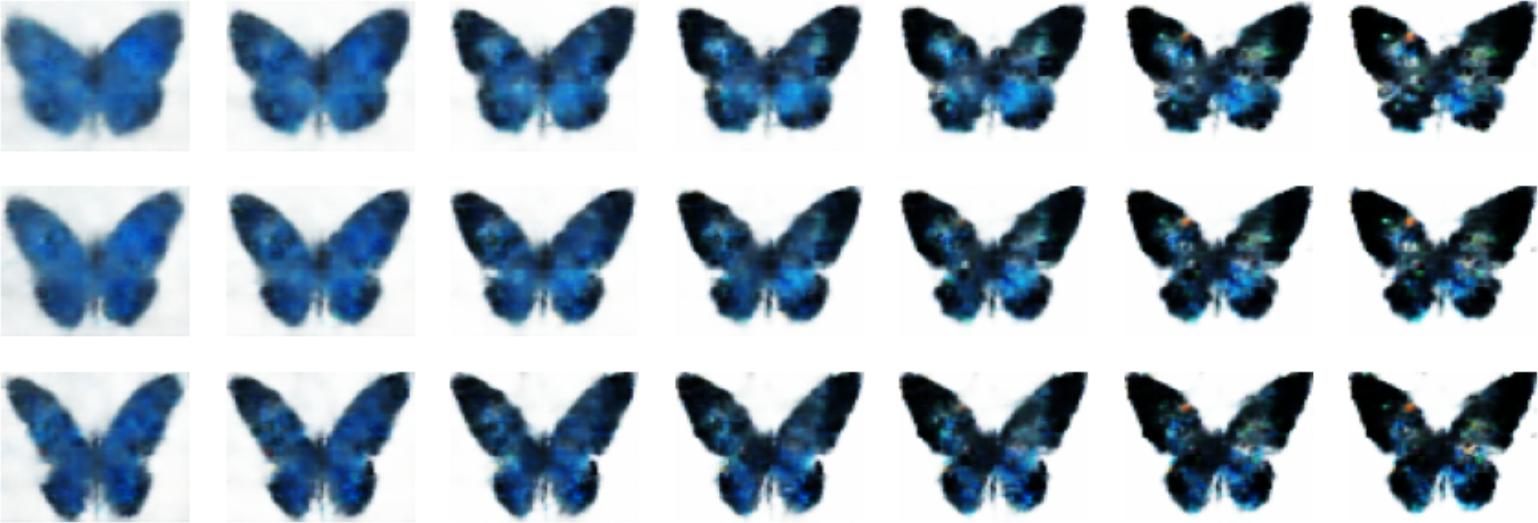
\includegraphics[width=10cm, height=4cm]{./fig/bm-vae.png}
    \caption{VAEs: Butterfly \& Moth Data}
    \label{fig:vae-bm}
\end{figure}
\par~\\
\textbf{GANs}. We visualize the outputs of linear interpolation in the same way as VAEs. We change the 1st, 120th, and 126th coordinates for MNIST data to obtain different numbers. Figure \ref{fig:gan-mnist} shows the generated images. For Butterfly \& Moth data, we change the 40th coordinate, which is related to the color and the posture of the butterfly. Figure \ref{fig:gan-bm} shows the generated butterfly.
\begin{figure}[!ht]
    \centering
    
\includegraphics[width=10cm, height=1cm]{./fig/gan-1.png}
    
\includegraphics[width=10cm, height=1cm]{./fig/gan-2.png}
    
\includegraphics[width=10cm, height=1cm]{./fig/gan-3.png}
    \caption{GANs: MNIST Data}
    \label{fig:gan-mnist}
\end{figure}
\begin{figure}[!ht]
    \centering
    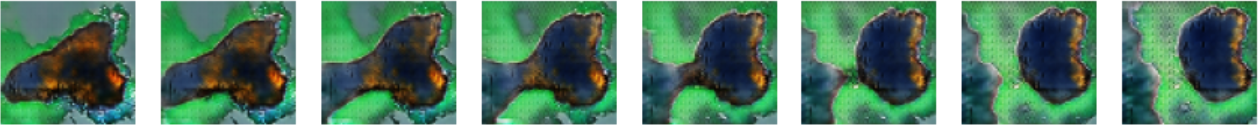
\includegraphics[width=10cm, height=1cm]{./fig/gan-bm.png}
    \caption{GANs: Butterfly \& Moth Data}
    \label{fig:gan-bm}
\end{figure}

\subsection{Discussion: Model Comparison}
CAEs are autoencoders that apply the CNN architecture to compress the input images into a lower dimensional latent space and reconstruct the images from the learned latent space. Using an encoder/decoder structure enables CAEs to capture as much information about data as possible, even without labels. However, CAEs are deterministic. That means there is a one-to-one relationship between the input and output in CAEs. Therefore, CAEs can't generate new samples. Based on the architecture of the traditional autoencoder, VAEs introduce randomness into the model by assuming a prior distribution of latent space and infering the posterior distribution during the training process. In most cases, we choose the standard Gaussian distribution as prior distribution, which helps the latent space to be complete and continuous. The probabilistic nature allows VAEs to generate new images from random noise.\par
GANs are designed for generating new samples. Instead of inferring the distribution of latent space, GANs sample from random noise and learn a transformation to imitate the real distribution of data. Gans improve the quality of imitations by training a discriminator to distinguish between generated samples and real samples.\par
In summary, VAEs sample from a prior distribution and infer the real distribution of latent space, while GANs sample from random noise and learn the data transformation by encouraging the competition between generator and discriminator.

\section*{Contributions}
\begin{tabular}{ll}
    \textbf{Name} & \textbf{Contribution}\\
    Chenyu Shi & Task 2 code, Task 2 report.\\
    Shupei Li & Task 3 code, Task 3 report, Task2 code.\\
    Shuang Fan & \\
\end{tabular}
\end{document}
